\label{s8} 

%\ssn{Learning Outcomes}
%After studying this week you will be able to:
%\begin{itemize}
%\item find probabilities for the normal distribution from tables;
%\item explain why the normal distribution is ubiquitous in practical problems; 
%\item use the normal distribution to provide approximate answers to appropriate problems. 
%\end{itemize}
%\end{n}

\subsection{The Gaussian Distribution}

\ssn{Motivating problems}
\begin{itemize}
\item I toss a coin a million times.  What is the probability that I get between 49.95\% and 50.05\% `heads'?  (Yes, in principal it's just a binomial distribution, but do you want to add up 1,000 terms?) 
\item More generally, can we say something more about the average  $Y = (X_1 + X_2 + \dots + X_n)/n$ of $n$ independent, identically distributed random variables?  Previously we encountered the Weak Law of Large Numbers and Chebychev's inequality which tell us something. But can we say anything about the general shape of the distribution rather than just the mean and variance? 
\end{itemize}
\end{n}

\ssn{Integration fact and some consequences}
Although one cannot specify an indefinite integral of $e^{-x^2}$ in terms of elementary functions, in SVCDE we show that  
\[ 
    \int_{-\infty}^\infty e^{-u^2} \dd u = \sqrt{\pi}.  
\]
(Alternatively, substitute $v = u^2$ to get the integral in terms of the gamma function.) 
Substituting $ u=x/\sqrt{2\sigma^2}$ (where $\sigma>0$ is a constant) we obtain 
 \[
     \int_{-\infty}^\infty e^{-\frac{x^2}{2\sigma^2}} \dd x =
     \sqrt{2\pi} \; \sigma. 
 \]
Differentiating both sides with respect to $\sigma$ we get\footnote{Alternatively integrate the integral below by parts, but the trick of differentiating with respect to a parameter is worth knowing!}
 \[
   \int_{-\infty}^\infty \frac{x^2}{\sigma^3}\, e^{-\frac{x^2}{2\sigma^2}} \, \dd x =
     \sqrt{2\pi}.  
 \]
Dividing by $\sqrt{2\pi}$ and setting $\sigma=1$ we get 
 \[
     \frac{1}{\sqrt{2\pi}}  \int_{-\infty}^\infty e^{-\frac{x^2}{2}} \, \dd x = 1 \qquad \text{and} \qquad  
       \frac{1}{\sqrt{2\pi}}  \int_{-\infty}^\infty x^2 e^{-\frac{x^2}{2}} \, \dd x = 1. 
 \]
\end{n}

\ssn{The standard normal distribution} \hfill 
\tcb 
We say the random variable $X$ has a \emph{standard normal distribution} if 
 \[
       f_X(x) = \frac1{\sqrt{2\pi}} \, e^{-\frac{x^2}{2}}. 
 \]
It has expected value zero and variance one.  
\etcb 

\begin{proof}
The two results at the end of the last item tell us that $f_X(x)$ is a probability density function and $\EE(X^2)=1$. Also, $\EE(X)=0$ because $f_X$ is symmetric about the origin. So $\var(X) = \EE(X^2) - (\EE(X))^2 = 1$. 
\end{proof}
\end{n}

\ssn{Proposition} \label{ltrrv}
Let $X$ be a continuous random variable and let $a,b$ be constants with $a>0$.   Then the pdf of $a X + b$  is given in terms of the pdf of $X$ by 
 \[
      f_{aX+b}(x) = \frac1a f_X
      \left( \frac1a(x-b) \right) .
 \]
The random variable $aX+b$ has $\EE(aX+b) = a \EE(X) + b$ and $\var(aX+b) = a^2 \var(X)$.  

\begin{proof}
We work with cumulative distributions: 
\begin{eqnarray*}
  F_{aX+b}(x) &=& \PP( aX+b \leq x ) \\
      &=&  \PP(aX \leq x-b) \\
      &=&  \PP\left( X \leq \frac1a (x-b)\right) \\ 
      &=&  F_X\left( \frac1a (x-b)\right).
\end{eqnarray*}
Differentiating both sides gives the required result.   The result about the expectation and variance are repeated from \ref{linev}. 
\end{proof}
\end{n}


\ssn{The general normal distribution}
Let $\mu$ and $\sigma>0$ be constants.  A random variable $X$ is said to have a \emph{normal distribution with parameters $\mu, \sigma^2$} and we write $X \sim \norm(\mu,\sigma^2)$ if it has pdf 
\tcb 
 \[
 f_X(x) = \frac1{\sqrt{2\pi\sigma^2}} \;
  e^{-\frac{(x-\mu)^2}{2\sigma^2}}. 
 \]
  Such a random variable has $\EE(X)= \mu$ and variance $\var(X)= \sigma^2$. 
 \etcb 
 
 \noindent 
  The standard normal distribution above is $\norm(0,1)$. 
\begin{proof}
The fact that this defines a pdf and that the expected value and variance are as stated follows from  fact (easily checked from \ref{ltrrv} above) that if $Z$ has standard normal distribution then $\sigma Z + \mu$ has $\norm(\mu,\sigma^2)$ distribution. 
\end{proof}
\end{n}

\ssn{Definition: standard deviation} \hfill 
\tcb 
The square root of the variance of a random variable is called the \emph{standard deviation} and is usually denoted $\sigma$ as above. 
\etcb 

\noindent The variance has good theoretical properties (such as $\var(X+Y) = \var(X) + \var(Y)$ when $X$ and $Y$ are independent), but the standard deviation is a better measure of the extent to which a distribution clusters around its expected value. 
\end{n}

\ssn{Visualising normal distributions}
\begin{figure}[h]
\centering
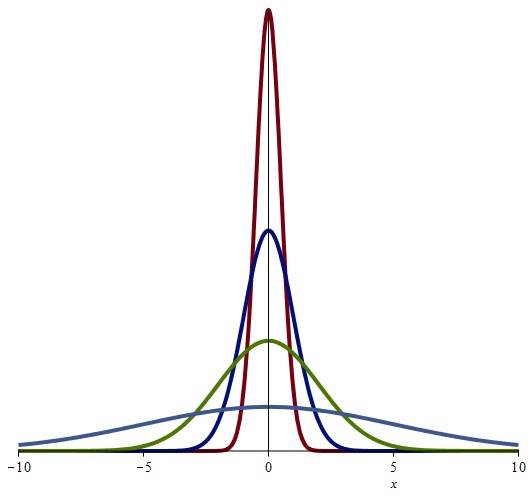
\includegraphics[width=0.4\textwidth]{images/normal_sd.png} 
 \qquad\qquad 
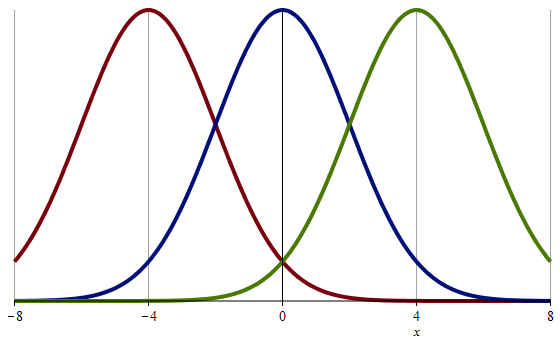
\includegraphics[width=0.4\textwidth]{images/normal_m.png}
\caption{Left: pdf of $\norm(0,\sigma^2)$ for $\sigma= 0.5, 1, 2, 5$. Right: pdf of $\norm(\mu,4)$ for $\mu=-4,0,4$. \label{normp}}
\end{figure}
The normal distribution is a familiar, symmetric ``bell-shaped curve'' centred on $\mu$.  The smaller $\sigma$ is the narrower the peak and therefore the greater likelihood of the random variable having a value close to the mean.  These features are clear in Figure~\ref{normp}. 
\end{n} 

\subsection{The Central Limit Theorem}

\ssn{The Central Limit Theorem}
The central limit theorem is the first big theorem of probability theory and plays a central role in applications. It's proof is beyond the scope of this course, and we will not even make a precise statement.  The idea however is important. 

\tcb
Consider a sequence of independent, identically distributed (i.i.d.) random variables $X_1, X_2, \dots$ each with mean $\mu$ and variance $\sigma^2$.  We know from \ref{wlln0} that the ``average of the first $n$''
 \[
   \bar{X}_n = \frac1n (X_1 + X_2 + \dots + X_n) 
 \]
has $\EE(\bar{X}_n) = \mu$ and variance $\var(\bar{X}_n) = \sigma^2/n$. 

The central limit theorem states that 
$$ \frac{ \bar{X}_n - \EE \bar{X}_n }{ \sqrt{\var(\bar{X}_n)} } \stackrel{\text{approx.}}{\sim} \norm(0,1)$$
for large $n$.
\etcb 

Note that there are many equivalent statements. Denote with $\Phi$ the cdf of the standard normal distribution, i.e.\ of $\norm(0,1)$, then
\begin{itemize}
    \item $\PP (\frac{ \bar{X}_n - \EE \bar{X}_n }{ \sqrt{\var(\bar{X}_n)} } \leq x ) \approx \Phi (x)$,
    \item $\PP \left( \sqrt{n} \frac{\bar{X}_n - \mu}{\sigma}  \leq x \right) \approx \Phi ( x )$,
    \item $\PP \left( \frac{\sum_{i=1}^n X_i - \EE \sum_{i=1}^n X_i}{\sqrt{\var(\sum_{i=1}^n X_i)}} \leq x \right) \approx \Phi ( x )$,
    \item $\PP \left( \frac{\sum_{i=1}^n X_i - n \mu}{\sqrt{n}\sigma} \leq x \right) \approx \Phi ( x )$,
    \item $\PP \left( a \leq \frac{\sum_{i=1}^n X_i - n \mu}{\sqrt{n}\sigma} \leq b \right) \approx \Phi ( b ) - \Phi(a)$.
\end{itemize}
\end{n}


%\ssn{Use of Central Limit Theorem}
%A practical application is that for large enough $n$, we can approximate $\bar{X}_n$ as having distribution $\norm(\mu , \sigma^2/n)$. 
%\end{n}

\ssn{Visualization of Central Limit Theorem}
Figure~\ref{fig:clt_plot} illustrates the application of the CLT for different sample sizes $n$ when applied to iid. Exponential rvs, $X_i\sim\text{Exp}(1)$ for $i=1,\ldots,n$. The expectation for this Exponential rv is $\mu=\EE{X_i}=\frac{1}{\lambda}=1$ and and its variance is $\var{X_i}=\frac{1}{\lambda^2} = 1$. As the sample size increases, we can see that the pdf for the sample mean, $f_{\bar{X}}(x)$ (solid line), becomes more symmetric and bell-like in shape until it is visually indistinguishable from the corresponding Normal approximation (dashed line) for the given sample size, i.e. $\bar{X}_n \stackrel{\text{approx.}}{\sim} \norm(1,\frac{1}{n})$ when $n$ is large.

\begin{figure}[!h]
    \centering
    \resizebox{\textwidth}{!}{\begin{tikzpicture}[
    declare function={gamma(\z)=
    (2.506628274631*sqrt(1/\z) + 0.20888568*(1/\z)^(1.5) + 0.00870357*(1/\z)^(2.5) - (174.2106599*(1/\z)^(3.5))/25920 - (715.6423511*(1/\z)^(4.5))/1244160)*exp((-ln(1/\z)-1)*\z);},
    declare function={gammapdf(\x,\a,\b) = \b^\a * \x^(\a-1) * exp(-\x*\b) / (gamma(\a));},
    declare function={ExpCLTpdf(\x,\n) = gammapdf(\x*\n,\n,1)*\n;},
    declare function={gauss(\x,\m,\s) = exp(-(\x-\m)^2/(2*\s^2)) / (2.506628*\s);}
]

\begin{groupplot}[
    group style={rows=1,columns=4},
    axis lines=left,
    enlargelimits=upper,
    samples=30,
    xlabel = {\Large $x$},
    ylabel = {\Large Density},
    ymax=2.3,
    ymin=0,
    every axis plot/.append style={ultra thick}
]

\nextgroupplot[title = \huge (a)]
\addplot [smooth, domain=0:3] {ExpCLTpdf(x,1)};
\addplot [smooth, domain=0:3,dashed]
{gauss(\x, 1, sqrt(1/1))};

\nextgroupplot[title = \huge (b)]
\addplot [smooth, domain=0:3] {ExpCLTpdf(x,5)};
\addplot [smooth, domain=0:3,dashed]
{gauss(\x, 1, sqrt(1/5))};

\nextgroupplot[title = \huge (c)]
\addplot [smooth, domain=0:3] {ExpCLTpdf(x,15)};
\addplot [smooth, domain=0:3,dashed]
{gauss(\x, 1, sqrt(1/15))};

\nextgroupplot[title = \LARGE (d)]
\addplot [smooth, domain=0:3] {ExpCLTpdf(x,30)};
\addplot [smooth, domain=0:3,dashed]
{gauss(\x, 1, sqrt(1/30))};

\end{groupplot}
\end{tikzpicture}
} 
    \caption{Application of the Central Limit Theorem to independent Exponential ($\lambda=1$) random variables with sample sizes (a) $n=1$, (b) $n=5$, (c) $n=15$ and (d) $n=30$. Solid line: Probability density function for the sample mean, $f_{\bar{X}}(x)$. Dashed line: approximate Normal distribution.}
    \label{fig:clt_plot}
\end{figure}

\end{n}

\ssn{And now the bad news}
The problem with the normal distribution is that one cannot explicitly integrate the pdf.  We solve this in two stages. 
\begin{enumerate}[(A)] 
\item 
\tcb 
If $X \sim \norm(\mu, \sigma^2)$ then 
 \[
       Z =    \frac1\sigma ( X - \mu) 
 \]
 has $\norm(0,1)$ distribution. 
 \etcb 
 
 \noindent This process of using this transform is often referred to as ``calculating a $Z$ value''.
 \item We use a table of values  (or calculator, etc) to look up values for the cumulative distribution function of $\norm(0,1)$, a function that we normally denote by $\Phi$.  So 
\tcb   \[
     \Phi(z) =  
     \frac1{\sqrt{2\pi}}\int_{-\infty}^z e^{-\frac{x^2}{2}}\dd x.
  \]
 \etcb 
 
 \noindent 
 We then calculate for $a\leq b$: 
   \[ 
   \PP( a \leq Z \leq b) = \Phi(b) - \Phi(a). 
   \]
 For negative values of $z$ we use $\Phi(-z) = 1-\Phi(z)$.  
 A stripped down set of tables that will be enough for us is found in Tables \ref{ntable} and \ref{ntable2}
\end{enumerate}
\end{n}

\begin{table}[h]
\centering
\begin{tabular}{|c|cccccccccc|}
 \hline 
 $\Phi(z)$  & 0.0&0.1&0.2&0.3&0.4&0.5&0.6&0.7&0.8&0.9  \\ 
   \hline 
0+& .5000 & 
.5398 & 
.5793 & 
.6179 &
.6554 &
.6915 &
.7257 &  
.7580 & 
.7881 & 
.8159  \\
1+& .8413 &
.8643 &
.8849 &
.9032 &
.9192 &
.9332 &
.9452 &
.9554 &
.9641 &
.9713 \\
2+& .9772 &
.9821 &
.9861 &
.9893 &
.9918 &
.9938 &
.9953 &
.9965 &
.9974 &
.9981 \\
3+ & .9987 &
.9990 &
.9993 &
.9995 &
.9997 & .9998& .9998 & .9999 & .9999 & .9999 \\
\hline 
\end{tabular}
\caption{\label{ntable} Values of $\Phi(z)$ for $0 \leq z < 4$ in steps of $0.1$. (Use $\Phi(-z)=1-\Phi(z)$ for negative values.)}
\end{table}

\begin{table}[h]
\centering
\begin{tabular}{|c|cccccc|}
 \hline 
 $\Phi(z)=$ & 0.9000 & 0.9500 & 0.9750 & 0.9900 & 0.9950 &0.9990     \\
 $z=$ &   1.283 & 1.645 & 1.960 & 2.326 & 2.576 & 3.090 \\
 \hline 
\end{tabular}
\caption{\label{ntable2} Values of $z$ with particular useful values of $\Phi(z)$.}
\end{table}

\ssn{Example}  
Let $X$ be normally distributed with $\mu = 3$ and $\sigma = 2$.  Evaluate 
$\PP( 1 < X < 2)$.

Here 
 \[
    Z = \frac{X-\mu}{\sigma} = \frac{X-3}{2}.
 \]
So $X=1$ and $X=2$ correspond to $Z=-1$ and $Z=-1/2$ respectively. So we want
 \[
  \PP(-1 < Z < -1/2) = \Phi(-1/2) - \Phi(-1) = 
   ( 1 - \Phi(1/2)) - ( 1- \Phi(1)) \approx 0.1498. 
 \]
\end{n}



\sse
In Fig.\ \ref{normp}, identify which graph corresponds to which values of $\mu$ and $\sigma$. 
\end{e}

\sse 
Let $X$ be normally distributed with $\mu = 3$ and $\sigma = 2$.  Evaluate 
$\PP( 1 < X < 2)$.  
\end{e}



\ssn{Example} 
We are now in a position to answer the first motivating question: I toss a coin a million times; what is the probability that I get between 49.95\% and 50.05\% `heads'?  

The number of heads we get is a random variable $X$ binomial distribution with $n=10^6$ and $p=1/2$.  The binomial distribution is an average of $n$ Bernoulli trials (tossing a single coin and counting how many heads), each of which has expected value $p=1/2$ and variance $p(1-p) = 1/4$.  The expected value and variance of $X$ are thus 
 \[
 \EE(X)= np = 500,000;  \qquad \var(X) = \sigma^2 = np(1-p) = 250,000,   
 \]
(which are facts about the binomial distribution we knew previously). 
Also, $\sigma = 500$.  

Having a look at the Central Limit Theorem, we can rewrite the sought probability as
\begin{align*}
\PP ( 0.4995 \cdot n \leq X \leq 0.5005 \cdot n)
&= \PP ( \frac{ 0.4995 \cdot n - \EE X }{\sqrt{\var (X)}} \leq \frac{ X - \EE X }{\sqrt{\var (X)}} \leq \frac{ 0.5005 \cdot n - \EE X }{\sqrt{\var (X)}}
\\ &
= \PP ( \frac{ -500 \cdot n }{500} \leq \frac{ X - \EE X }{\sqrt{\var (X)}} \leq \frac{ 500 }{500}
\\ &
\approx \Phi(1)- \Phi(-1) 
\\ &
= 2 \Phi(1) - 1 
\\ &
\approx 0.682.
\end{align*}
However, since $X$ takes discrete values, while we are approximating with a continuous distribution, we might want to make a ``continuity correction'' to improve our result. 
  So e.g.\ we associate the discrete value of 499500 heads with the range $[499499.5, 499500.5]$ in the normal distribution. (You will not lose marks in this course if you neglect this and quite often we specifically ask you not to do this.)  
 Then our problem changes form whether $499500 \leq X \leq 5005$ to 
$ 499499.5 \leq X \leq 500500.5 $
 for our calculation, which changes the result to $2 \Phi( 1.001)-1$, which gives the same numerical result.


\noindent 
The transformation from $X$ values to $Z$ values is  
 \[
     Z = \frac1\sigma (X - \mu) = \frac1{500} (X - 500,000)
 \]
 and this takes $X=499499.5$ and $X=500500.5$ to something very close to $Z=-1$ and $Z=1$ respectively. 
 So the corresponding question about $Z$ is to find $\PP(-1 \leq Z \leq 1)$.  Thus our answer is 
  \[
   \Phi(1) - \Phi(-1) = \Phi(1) - (1-\Phi(1)) = 2 \Phi(1) - 1 \approx 0.682.
  \]
 (Useful rule of thumb: approximately 2/3 of a normal distribution is within one standard deviation of the mean.) 
 
I tried to check this answer with Wolfram alpha.   It gave me the following --- not sure how it added up lots of positive numbers and obtained something negative.  I guess this is why we use the normal approximation! 
\begin{figure}[h!] 
\centering
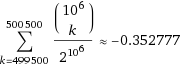
\includegraphics[]{images/wal.png}
\end{figure}
\end{n}

\ssn{Proposition}  \label{affnorm}
Let $X$ be a normal random variable with $\EE(X)=\mu, \var(X) =\sigma^2$.   Then given constants $a\not=0, b$ the random variable $Y=aX+b$ is also normally distributed with $\EE(Y)=a\mu +b$ and $\var(Y) = a^2 \sigma^2$. 
\begin{proof}
The fact that the expectation and variance are as claimed follows from general theory.  The verification that $Y$ is normal is a straightforward application of \S\ref{ltrrv}. (Exercise.) 
\end{proof}
We were implicitly assuming this result in the introductory reading. 
\end{n}

\ssn{Example: distribution of $Z^2$}
It is important in applications to understand the distribution of the square of a normally distributed random variable. Suppose that $Z$ is standard normal.   

Using the cumulative distribution trick again, 
 \[
 \PP( Z^2 \leq x ) = \PP( -\sqrt{x} \leq Z \leq \sqrt{z} ) 
  = 2 \PP( 0 \leq Z \leq \sqrt{z} ).  
 \]
Setting $X$ = $Z^2$ we therefore have 
 \[
   F_X(x) = \PP( X \leq \sqrt{x}) = \frac2{\sqrt{2\pi}} \int_0^{\sqrt{x}} e^{-z^2/2} \dd z
  \]
 and so 
 \[
  f_X(x)  = \frac{\dd}{\dd x} 
  \left(  \frac2{\sqrt{2\pi}} \int_0^{\sqrt{x}} e^{-z^2/2} \dd z  \right) = 
   \frac2{\sqrt{2\pi}} e^{-x/2} \frac{\dd}{\dd x} \sqrt{x} = 
    \frac1{\sqrt{2\pi}} x^{-1/2}  e^{-x/2}.
 \]
The fact that this is a constant times $x^{-1/2} e^{-x/2}$ means this must be the gamma distribution with $\alpha = \lambda = 1/2$. 
\end{n}

\ssn{The $\chi^2$ and other distributions (optional)}
Because of the Central Limit Theorem, a lot of basic statistics rests on normal distributions: data is often assumed to have come from sampling from a normal distribution unless there is evidence otherwise.  The $\chi^2$ distribution with $n$ degrees of freedom is precisely the sum of the squares of $n$ independent standard random variables. (So above we showed that $\chi^2(1) \sim \gamm(1/2,1/2)$.)   Other well-used distributions include the $F$-distribution which is (up to a scale) a quotient of two $\chi^2$ random variables and Student's t-distribution which measures the distribution of the mean of a sample from a normal distribution. 

Returning to $\chi^2$, let us try and understand $\chi^2(2)$.  If we have a unit normal random variable $X$ then for a small increment $\Delta x$ in $x$ we have
 \[
      \PP( x \leq X \leq x+ \Delta x) \approx f_X(x) \Delta x = 
       \frac1{\sqrt{2 \pi}} e^{-x^2/2} \Delta x.
 \]
If we have another independent normal random variable $Y$ then 
 \[
    \PP( x \leq X \leq x+ \Delta x \,\text{ and } \, 
     y \leq Y \leq y + \Delta y) \approx 
      \frac{1}{2 \pi} e^{-(x^2 + y^2)/2} \Delta x \, \Delta y.
 \]
Thus we have what we will soon call ``joint density function'' 
 \[
       f_{X,Y}(x,y)  = \frac1{2\pi}  e^{-(x^2+y^2)/2}
 \]
that can be integrated to calculate the probability of the ``random point'' $(X,Y)$ lying in a given area of the $(x,y)$-plane.

In particular, we can use this to calculate the cumulative distribution of $X^2+Y^2$ by converting to polar coordinates:
\begin{eqnarray*} 
     F_{X^2+Y^2}(t) &=&  \PP( X^2+Y^2 \leq t) \\
       &=& \frac1{2\pi}  \int_{r=0}^{\sqrt{t}} \int_{\theta=0}^{2\pi} 
         e^{-r^2/2} r \dd \theta \dd r \\
      &=&  \int_{r=0}^{\sqrt{t}} 
        r  e^{-r^2/2}  \dd r  = \left[ - e^{-r^2/2}   \right]^{\sqrt{t}}_0  = 1 - e^{-t/2}.
\end{eqnarray*} 
We recognise this (or we differentiate) to obtain the density function 
 \[
     f_{X^2+Y^2}(t) = \frac12 e^{-t/2}
 \]
and so  $\chi^2(2) \sim \expo(-1/2)$ or equivalently $\gamm(1, 1/2)$.

\bpr 
Follow the above reasoning to deduce that $\chi^2(3) \sim \gamm(3/2, 1/2)$. You will need to substitute $u=r^2$ in the final integral to obtain a result in terms of the $\Gamma$-function.   

For a further challenge, consider higher values of $n$. 
\epr %\\end{e}

\end{n} % was above \bpr

\subsection{Exercises and problems} 
 

\sse 
In the ``million tosses'' problem, how likely is it that at least 50.1\% of the tosses come down ``heads''.    (Ans: 0.0228)
\end{e}
 
\sse 
In Problem~\ref{chebex} you were asked to calculate a value of $n$ such that  the probability that the proportion of heads is within $0.01$ of $0.5$ is at least $0.95$. (The result was that it requires $n\geq 200,000$.) 

Use approximation by a normal distribution to estimate the value of $n$ needed for this to be true.  
 \end{e}
 
\sss 
The number $N$ of heads in $n$ tosses is binomial $(n, 1/2)$ and so has expected value $n/2$ and variance $n/4$. The proportion of heads is $X= N/n$ which thus has expected value $1/2$ and variance $1/(4n)$. The $Z$-transformation is thus 
 \[
       Z = \frac{ X - 0.5}{1/(2\sqrt{n})}.
 \]
From tables, $\Phi(2) \approx 0.975$ and so 
 \[
 \PP(-2 \leq Z \leq 2) \approx 0.95.
 \]
For $|X-0.5|\leq 0.01$ to translate into $|Z| \leq 2$ we require 
 \[
         \frac{0.01}{1/(2\sqrt{n})} \geq 2
 \]
or $n \geq 10,000$. 
\end{s}
 
 
 
\sse 
Adapt the statement and proof of \S\ref{ltrrv} to cover the case $a<0$.
\end{e}

\sss 
The correct statement is 
 \[
      f_{aX+b}(x) = \frac1{|a|} 
      f_X\left( \frac1a(x-b) \right) .
 \]
For the proof, remember that when you multiply n inequality by a negative number, the direction reverses. 
\end{s}

\sse 
Complete the proof of \S\ref{affnorm}. 
\end{e}
